\documentclass[11pt]{standalone}

\usepackage{helvet}
\usepackage{units}
\usepackage{textcomp}

\usepackage{ifthen}
\usepackage{tikz} 
\usetikzlibrary{shapes.misc}
\usetikzlibrary{arrows,arrows.meta}
\usetikzlibrary{calc,intersections, patterns, math}
\usetikzlibrary{decorations.pathmorphing}
\usetikzlibrary{shapes.geometric}

\definecolor{pfeil}{RGB}{168,167,167}
\definecolor{petrol}{RGB}{0, 118, 136}
\definecolor{blue}{RGB}{0, 118, 136}
\definecolor{white}{RGB}{35,35,35}
% \definecolor{blue}{RGB}{100, 100, 255}
\definecolor{darkgoldenrod}{RGB}{184, 134, 11}
\colorlet{petrol-lighter}{petrol!40}
\colorlet{darkgoldenrod-lighter}{darkgoldenrod!40}
\definecolor{background}{RGB}{35,35,35}

\begin{document}

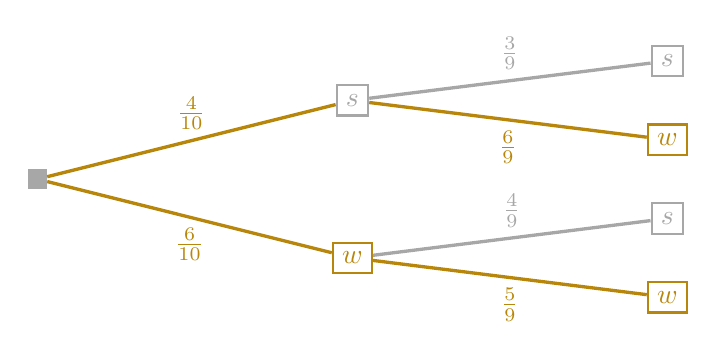
\begin{tikzpicture}[pfeil, xscale=1, yscale=0.25]

	% Stufe 1
	\node[draw,fill] (S) at (0,0) {};
	
	\node[draw,rectangle, thick] (F1) at (4,4) {$s$};
	\node[draw,rectangle, thick,darkgoldenrod] (F2) at (4,-4) {$w$};
	
	\draw[very thick, darkgoldenrod] (S) -- node[above] {$\frac4{10}$} (F1);
	\draw[very thick, darkgoldenrod] (S) -- node[below] {$\frac6{10}$} (F2);

	% Stufe 2
	\node[draw,rectangle, thick] (F11) at (8,6) {$s$};
	\node[draw,rectangle, thick,darkgoldenrod] (F12) at (8,2) {$w$};
	
	\draw[very thick] (F1) -- node[above] {$\frac39$} (F11);
	\draw[very thick,darkgoldenrod] (F1) -- node[below] {$\frac69$} (F12);

	\node[draw,rectangle, thick] (F21) at (8,-2) {$s$};
	\node[draw,rectangle, thick,darkgoldenrod] (F22) at (8,-6) {$w$};
	
	\draw[very thick] (F2) -- node[above] {$\frac49$} (F21);
	\draw[very thick, darkgoldenrod] (F2) -- node[below] {$\frac59$} (F22);

	
\end{tikzpicture}




\end{document}
